\chapter{Extracting actionable entities for disaster response using semi-supervised learning}

\section*{Introduction}
% * Done
The previous three chapters have highlighted the importance of information in crisis management.
The first chapter introduces the notion of Common Operational Picture (COP).
The COP is a cartographic representation used by all response actors to facilitate their organization.
This map uses concepts that are common to all actors.
The third chapter, proposed concepts to support crisis management (Figure~\ref{information:information-models}).
The advantage of these concepts is that they can provide a computer representation of the crisis.
This allows the information related to these concepts to be manipulated automatically.
In particular, the third chapter highlighted two essential information needs for decision-makers: situational awareness and access to actionable information.
Having access to the right information at the right time is a critical need of the response actors.
Concurrently, social media are recognized as sources of information of interest.
However, they are complicated to process due to the volume of data, their heterogeneity, and uncertainties regarding the information they convey.
Organizations in charge of the response are therefore looking for tools to reduce the complexity of the processing.
This observation brings us to the second research question identified in the first chapter: \emph{How can the actionable information available on social be automatically retrieved during crisis response?}
Therefore, this chapter proposes a method to collect automatically actionable information for decision-makers.
The presented method is based on artificial intelligence and automatically retrieves the information presented in the previous chapter.
Figure 6 repeats the diagram presented in the first chapter (Figure 1) and highlights the scope of the contribution made in this chapter.

\begin{figure}[htb]
    \centering
    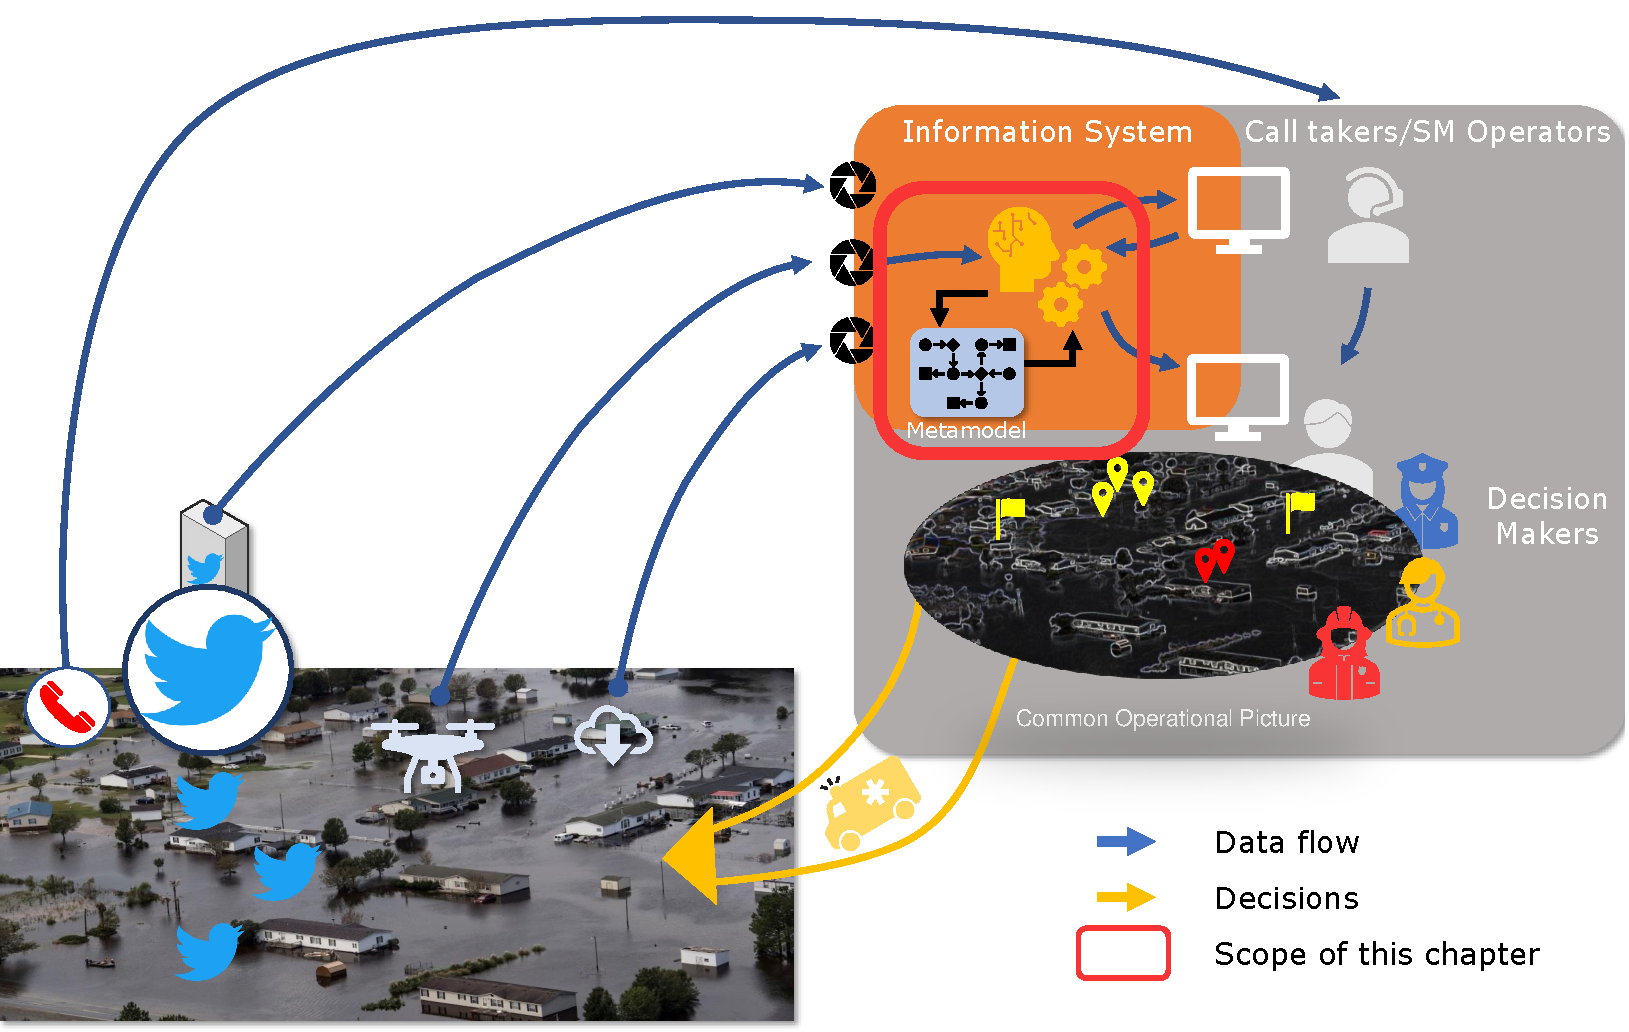
\includegraphics[width=\textwidth]{figures/chap-4/position-chapter.pdf}
    \caption{Location of this chapter in relation to the body of this manuscript.}
    \label{processing:big-picture-manuscrit}
\end{figure}

The proposed approach aims to collect information present in the information model proposed at the end of chapter 3 (see Figure~\ref{information:information-models}).
The method relies on machine learning to identify the information expected by decision-makers within the messages posted on social media.

Unlike most of the other approaches that process the social media information in this context, the processing is not performed at the scale of the message itself.
Instead, the message is processed at the scale of the different terms that compose the message.
The method relies on previous work realized on this topic to take the data further.
Figure~\ref{processing:social-media-processing} illustrates the positioning of our contribution in the light of previous work.

The chapter is organized into three sections.
The first section presents the business and technical constraints that emerge when retrieving this information.
The second section details the scientific foundations and the functioning of the proposed method.
Finally, the last section presents and discusses the results of the method on a test data set.

\section{Problem statement}
Chapitre 3 shown that most of the information retrieval is currently performed manually.
Dedicated operators are charged to identify relevant information coming from different information channels (reports, calls made to the call centers, news, social media, etc.).
However, social media raises new challenges due to the high volume of data and the noise/information ratio.
The literature review in Chapter 2 highlighted the trend toward automation in crisis informatics.
This trend is intended to reduce the monitoring burden that operators must bear to achieve their results.
In addition, crisis response is usually not an environment that leaves room for insufficiently effective resources.
The call takers have thus developed frameworks that allow them to obtain information aligned with the needs of the decision-makers.
The first section of Chapter 2 has already presented the most important systems designed for automatic social media processing.
The systems described all seek to simplify the processing of social media by the responders.
Automatic detection of information in a message stream is subject to constraints.

This section presents the environment in which the automated processing takes place.
In particular, two components are highlighted in dedicated sub-sections.
A technical component related to the use of machine learning is presented first.
Then a second part presents a business component that emphasizes the needs and constraints of recovering the actionable information in social media texts.

\subsection{Machine learning for disaster response}
Machine learning approaches rely on data to provide information to people who consume the results.
These approaches are generally composed of two phases.
The first phase refers to the step where data are used to train the machine learning model.
During this phase, the model learns the latent patterns in the data to produce its results.
To do so, the data provided are annotated, meaning that each data point is associated with a label.
Hence, the model learns to associate the data with the appropriate label.
Once the model is trained, it enters the inference or prediction phase.
In this phase, new, unseen data are provided to the model.
The machine learning then infers the label associated with the data provided.
There are then two types of data: labeled and unlabeled.
Different methods are used depending on the proportion of labeled data used in the training phase.
When the training set is entirely composed of labeled data, the approach is said supervised.
This approach is the one most often chosen when training a model.
However, it comes at the cost of having a set of data annotated.
Data annotation can be time-consuming, expensive (if trained professionals annotate them), or challenging when the labels used are too ambiguous.
The opposite is said unsupervised or self-supervised when the entire training set is unlabeled.
Nowadays, more and more tasks are handled using this approach, particularly in the case of large models.
The chosen approach trains the model by providing the label directly in a sentence.
For example, a model trained to translate text from English to French following this method would use sentences expressing the translation.
Thus, instead of providing the model with the couple ("potato," "patate"), the model receives the sentence "The word 'potato' is translated as 'patate' in french."
The last way to train a model is to use a semi-supervised approach where the training set is composed of two sets.
The first set comprises labeled data and the second one of unlabeled data.
This approach relies on the labeled data to identify the required information to learn.
Then, the unlabeled data are used to generalize the patterns learned to more data points.

The crisis informatic domain takes on the challenge to provide valuable tools to help process social media data.
To reduce the load on the operators, many approaches have been taken.
The first approach consists in increasing the processing capacity through the help of volunteers.
Crowdsourcing tools allow the former to help in the classification of the messages that can then be forwarded to decision-makers \parencite{imranAIDRArtificialIntelligence2014}.
A second approach is to lower the incoming flow of data that the operators are facing.
Some explored ways to reduce the noise part of the flow by filtering messages according to their relevance (linked or not to the ongoing event) \parencite{carageaClassifyingTextMessages2011,imranAIDRArtificialIntelligence2014}.
Others attempted to shrink the incoming flow as a whole by summarizing the information from the incoming data \parencite{rudraSummarizingSituationalTweets2016}.
\textcite{zahraAutomaticIdentificationEyewitness2020} proposed to identify direct eyewitnesses of events using a machine learning model trained in a supervised way.
The model, a Random Forest, uses features that the authors extracted manually to increase the performances of the model.
A common solution to most NLP problems nowadays is to fine-tune a pre-trained language model.
This approach associates a good ratio of performance/data labeled and can be performed on a reasonable amount of hardware to run.
However, this approach still requires a significant amount of labeled data, representative of the data that the model will process in the future.
This approach has already been used to classify the relevance of messages posted on social media \parencite{kozlowskiThreelevelClassificationFrench2020}.
The architecture of these models is synthesized in Figure~\ref{processing:social-media-processing}

\begin{figure}[htb]
    \centering
    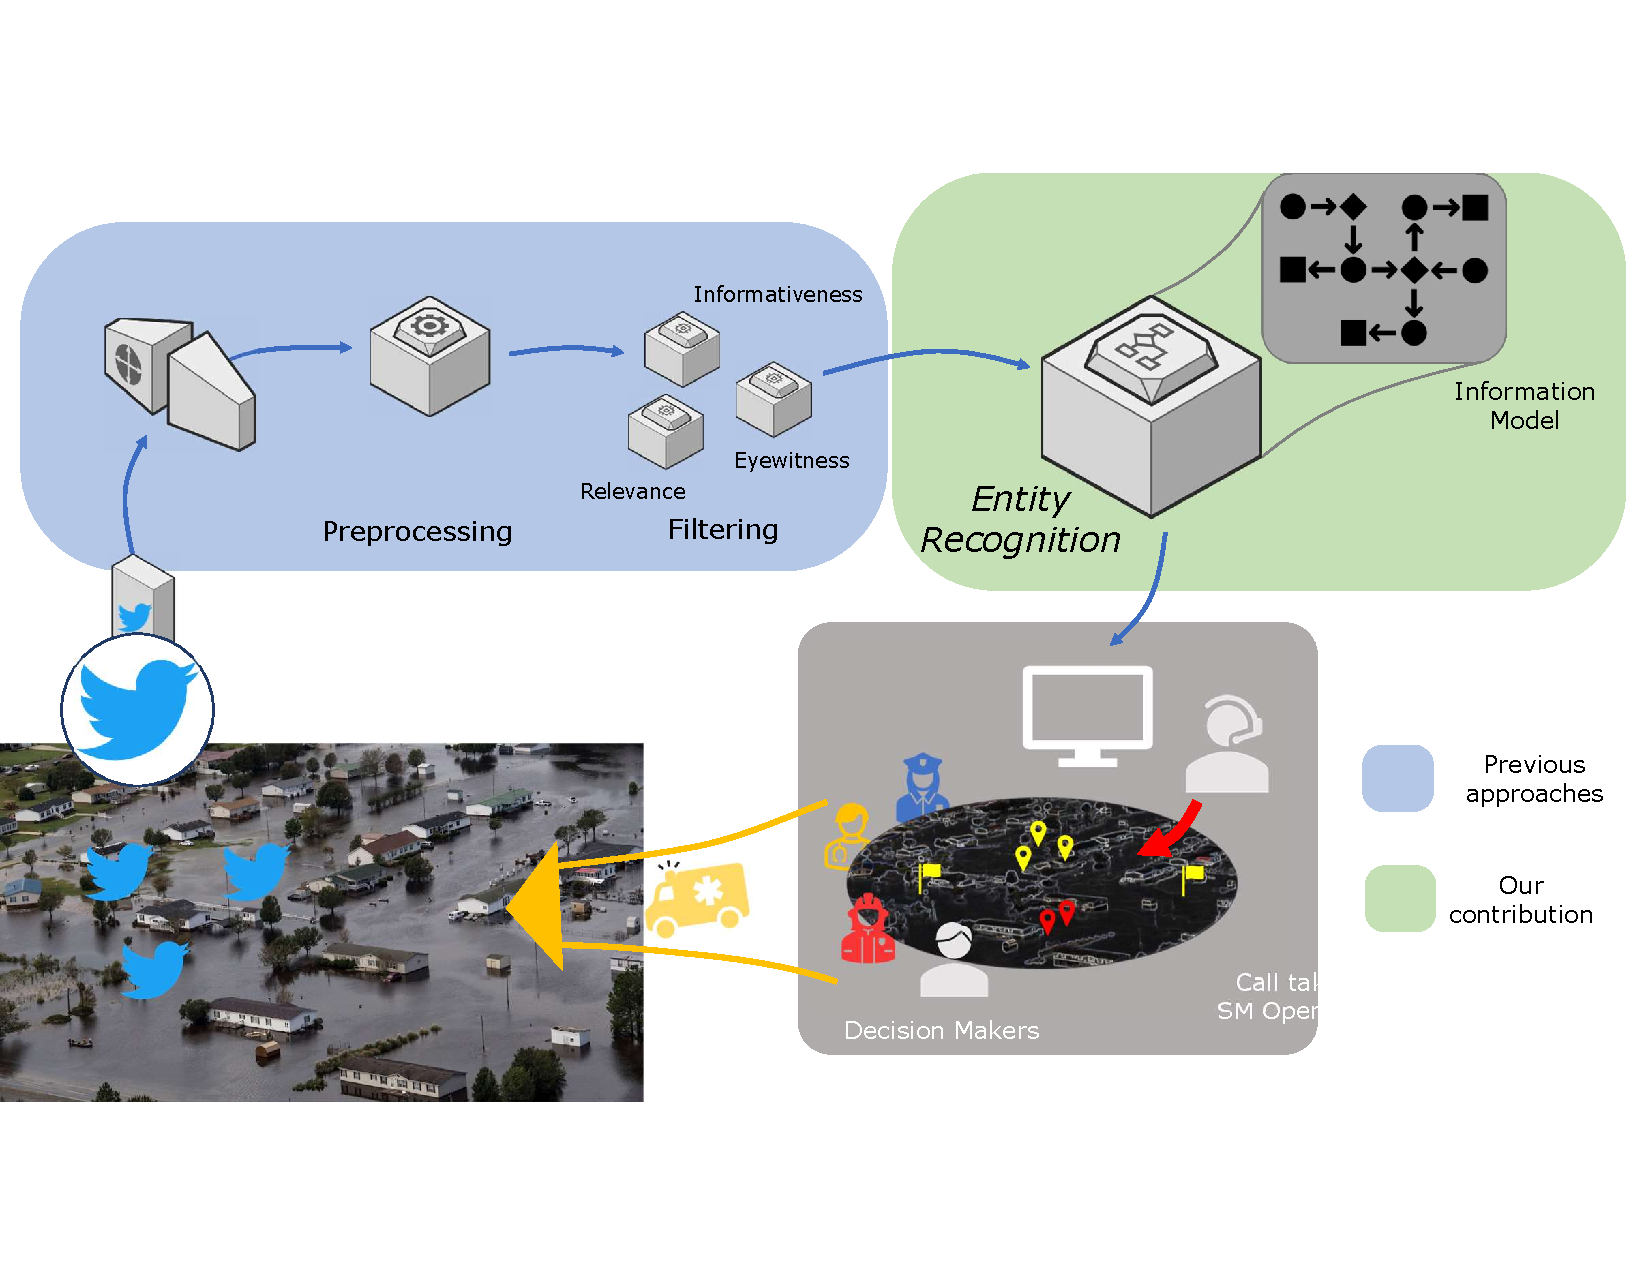
\includegraphics[width=\textwidth]{figures/chap-4/social-media-processing.pdf}
    \caption{Data processing pipeline used in most of social media processing tools.}
    \label{processing:social-media-processing}
\end{figure}

Most of the approaches used to deal with social media in crisis management are now based on supervised machine learning models.
These models are trained using publicly available data sets.
Most of the models are trained using sets such as the \emph{CrisisLexT26} \parencite{olteanuCrisisLexLexiconCollecting2014,olteanuWhatExpectWhen2015}.
However, these sets only offer labels associated with messages (composed of tweets posted on Twitter).
This means that they do not specify the content of each message, nor if there could be more than one piece of information contained in the message.
Thus, obtaining actionable information seems complex in the case of supervised learning for several reasons:

\begin{enumerate}
    \item The model is trained on past data, and there is no guarantee that the new data will be similar (especially in crisis management).
          However, disasters are, by nature, unpredictable.
          The model's performances can become uncertain in this context.
    \item Models are not explicable/interpretable, which can have consequences.
          It is essential to consider the user-machine relationship, especially in complex and/or stressful situations.
          The worst-case scenario would be that the system provides erroneous results and that the decision-makers still take into account, unaware of the errors.
          To avoid this scenario, \textcite{endsleyDesigningSituationAwareness2016} recommends including the operators in the functioning of the algorithm by allowing them to influence the results of the algorithm in the most intuitive way possible.
    \item If one wishes to retrain the model at the time of the crisis, it will require labeled data, which cannot necessarily be done.
\end{enumerate}

This observation, therefore, motivates the choice of a training method that is not supervised.
A self-supervised approach is not feasible in the case of named entity recognition.
Hence the choice of a semi-supervised model to recover actionable information.

\subsection{Issues raised by the context of disaster response}
Social media make a significant volume of data available through text, photos, or videos.
Processing social media content is tedious and more challenging when compared directly with phone calls.
Part of this challenge comes from the fact that most of the data are unrelated to the current event operators are interested in.
The challenges faced by potential social media operators are hence twofold.
First, they need to process the volume of incoming data.
Secondly, they need to screen each remaining message to identify the relevant information.
Therefore, the emergency staff is looking for tools to help them in their task.
The solution proposed hence need to solve two challenges:

\begin{itemize}
    \item It has to reduce the time spent processing incoming messages by reducing the number of unrelated messages and screening.
    \item It has to deliver value to the decision-makers by providing the information required by the different actors.
\end{itemize}

As shown previously, the first challenge has already been discussed significantly in the scientific literature.
Hence, the contribution made in this chapter builds on previous work and focuses on addressing the second part of the challenge.
Therefore, the goal is to highlight the information valuable information for decision-makers.
Here, valuable information refers to the concepts presented at the end of Chapter 3.
This objective is close to an NLP task, the Named Entities Recognition (NER).
NER is a classification problem that seeks to (i) locate and (ii) label the named entities (brand, person, organization, location, etc.) contained in a sentence.
The term "entity" is used rather than "word" to reflect that social media messages can be composed of other elements such as URLs, for example.
However, instead of looking for named entities, our approach aims to identify predefined entities, which are the different concepts of the information model.
This model is trained to perform this task using a semi-supervised learning approach to overcome the challenges presented in the previous section.
This approach taken is summarized in Figure~\ref{processing:social-media-processing-proposition}

\begin{figure}[htb]
    \centering
    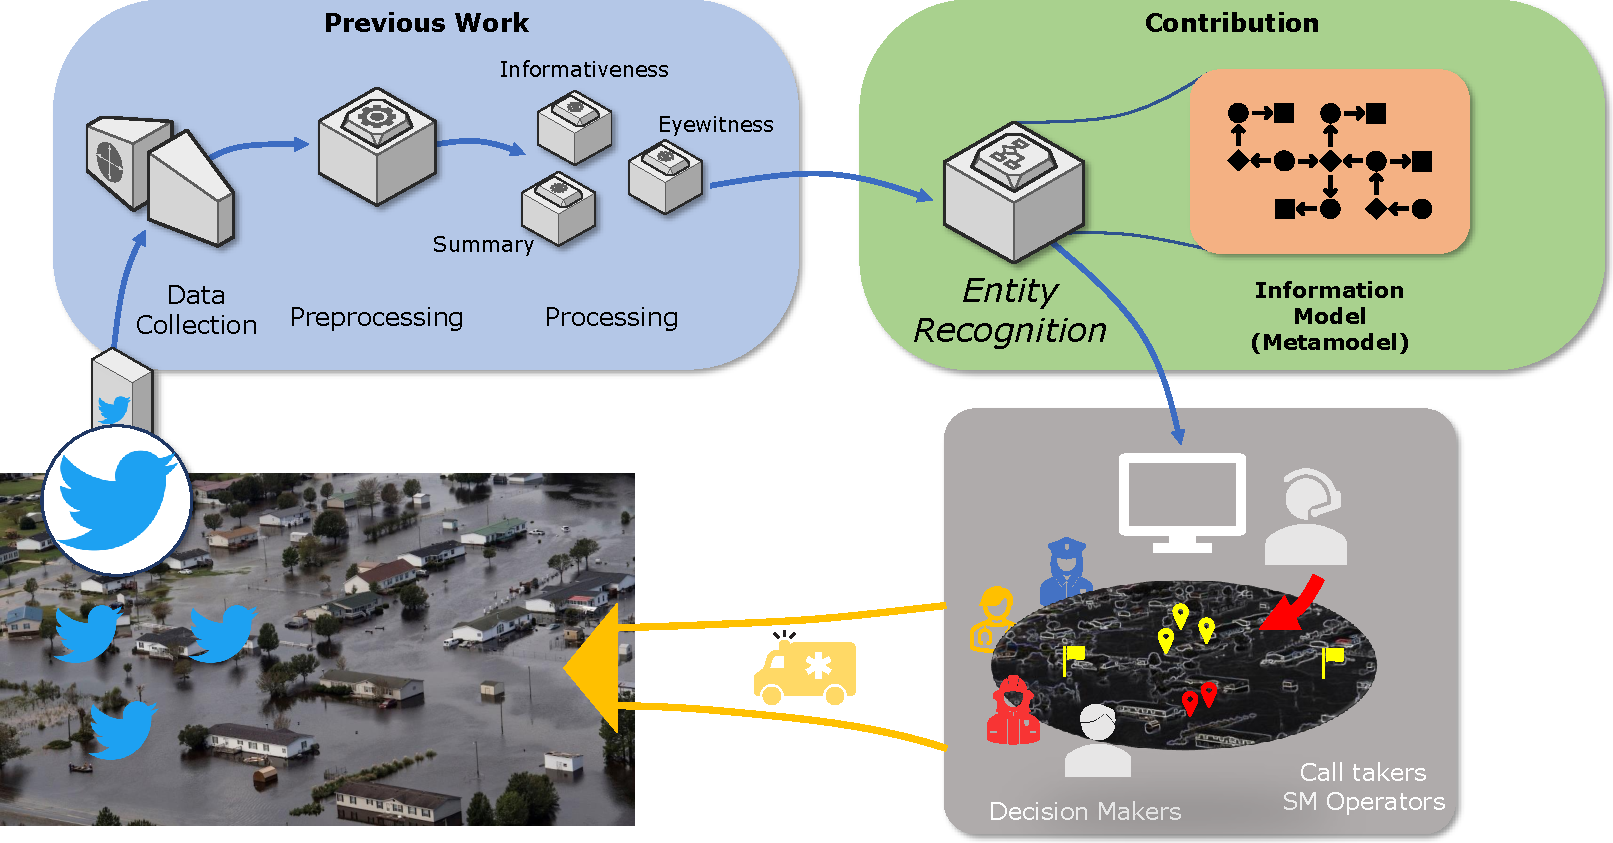
\includegraphics[width=\textwidth]{figures/chap-4/social-media-processing-proposition.pdf}
    \caption{Positioning of our contribution with respect to other social media processing tools.}
    \label{processing:social-media-processing-proposition}
\end{figure}

To summarize, the aim is to facilitate the processing of social media data.
This is achieved by highlighting the information decision-makers need, i.e., information in the information model presented at the end of Chapter 2.
The following part details the proposed solution, a machine learning model trained to recognize entities within a sentence.

\section{Scientific foundations of the approach}
The proposal is to train a machine learning model in a semi-supervised way to recognize the entities that belong to the different classes.
The approach relies on two properties of the most recent language models.
First, they allow encoding textual data into vectors.
In our case, each word, labeled or not, is associated with a vector.
Secondly, the word vectors are obtained to create a vector space.
This vector space has the property that the distance between the different vectors represents the semantic similarity between the words associated to the vectors.
The vector space thus contains clusters of vectors composed of semantically similar entities.
These vectors are obtained by processing the vector space data with a clustering algorithm.
It is from this step that the labeled data intervene in the method.
The terms labeled by the operators are included with the other terms.
Therefore, they appear in some of the clusters identified previously.
The labeled terms are used to associate the non-labeled content of the clusters with the labels.
The labels are then propagated from the labeled terms present in a cluster to the non-labeled terms.
In this way, the non-labeled terms semantically close to the labeled terms are associated with the different concepts we identify.
The different steps of the algorithm are outlined in Figure~\ref{processing:big-picture}.
The method is composed of four main steps after data normalization.
These are:

\begin{enumerate}
    \item Generation of the word vectors associated with each token.
    \item Dimension reduction of the vector space obtained previously to facilitate the following clustering.
    \item Identification of semantic clusters present in the vector space using a clustering algorithm.
    \item Label propagation within the different semantic clusters.
\end{enumerate}

\begin{figure}[htb]
    \centering
    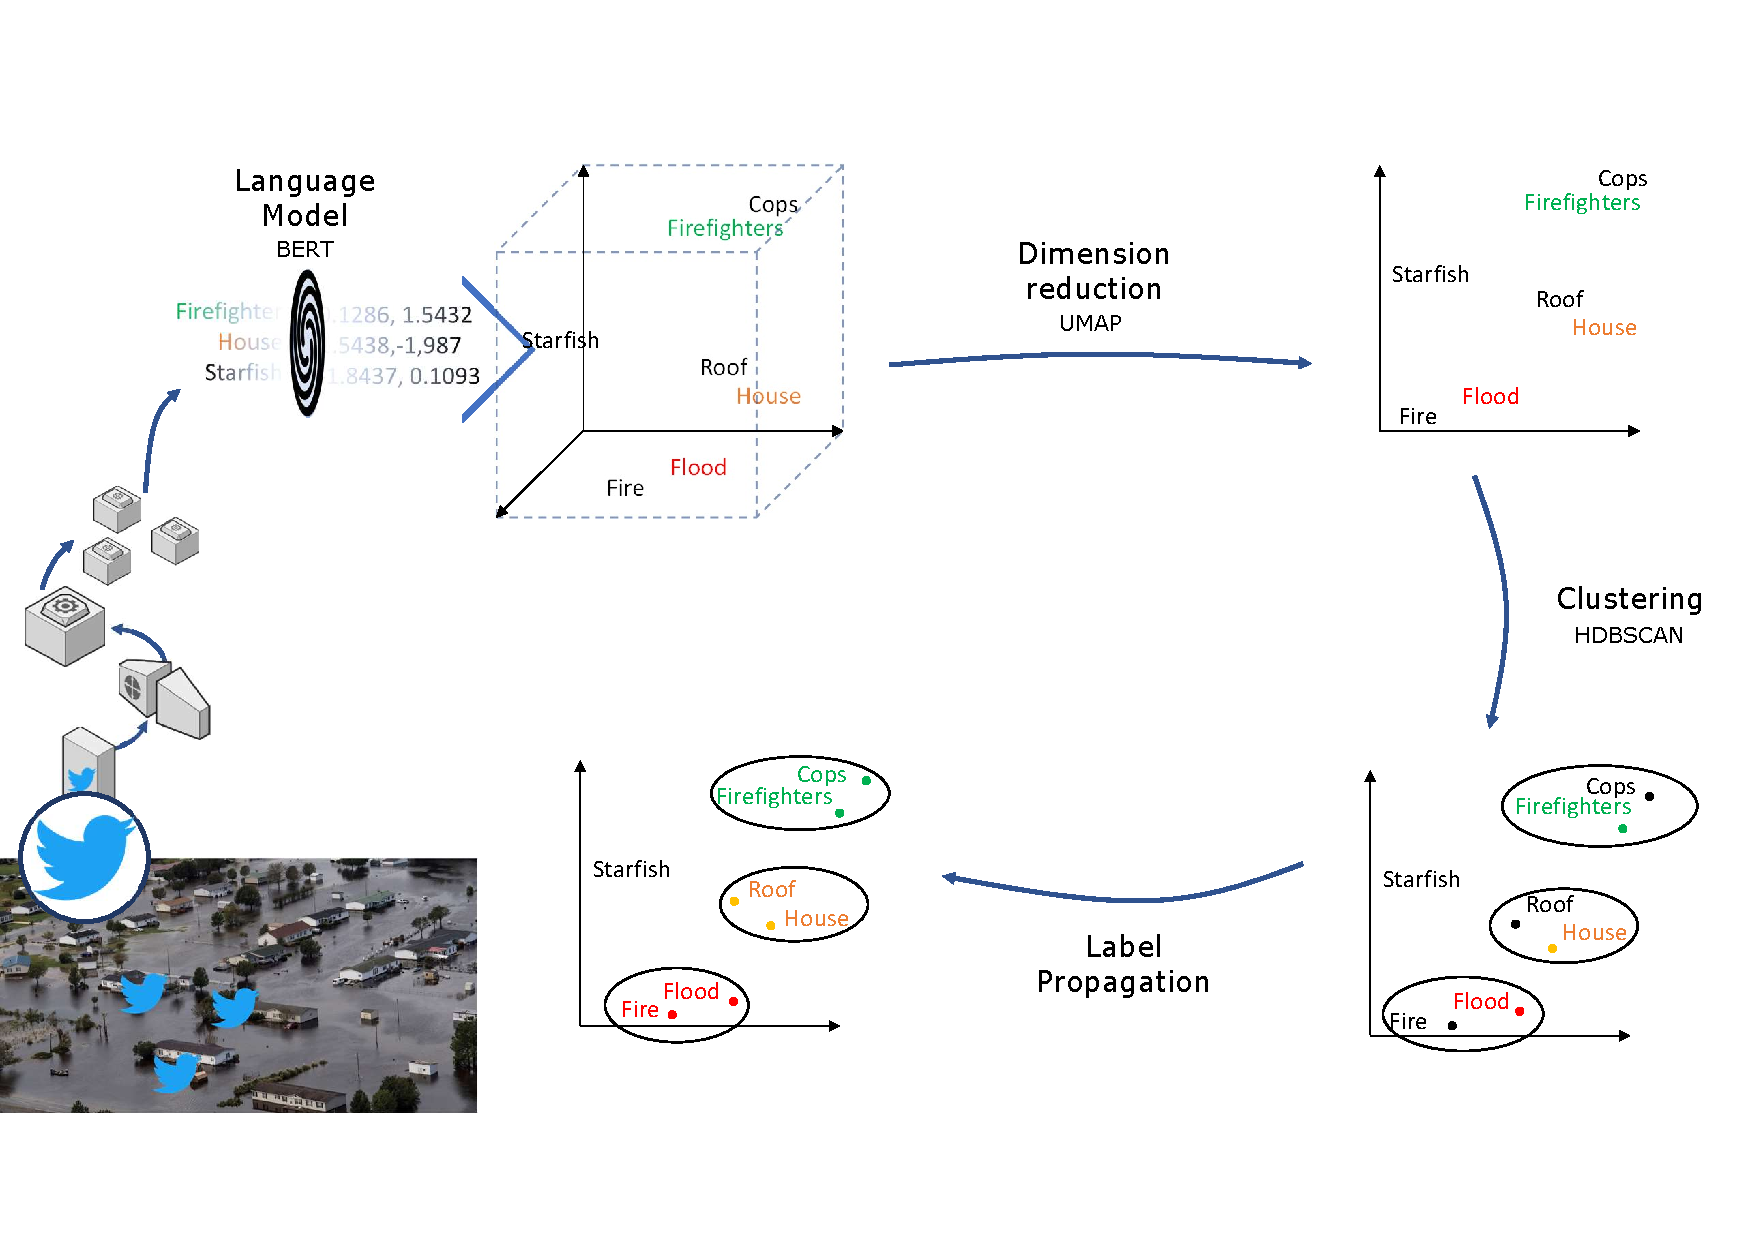
\includegraphics[width=\textwidth]{figures/chap-4/big-picture.pdf}
    \caption{Overview of the approach developped in this chapter. The colors associated with the dots and words correspond to the different information proposed in Figure~\ref{information:information-models}}
    \label{processing:big-picture}
\end{figure}

The semi-supervised approach implies that the training is made using two distinct datasets.
One dataset contains labeled data, and the other has unlabeled data.
The former, in our approach, contains text messages obtained from previous disaster events.
These messages are sliced to obtain a list composed of the entities that make up the message.
This process of breaking down sentences is called text \emph{tokenization}.
Unlabeled sentences are thus broken down into lists of corresponding tokens.
Once all messages are split, a vocabulary is created.
This vocabulary is composed of all the unique entities used in the original text messages.
The labeled dataset is composed of words/tokens paired with one of the information labels.
The two sets of tokens are then merged to create a set of unique tokens, where some are labeled.
The next section presents how language models convert these tokens to vectors that embed the semantic of each token.

\subsection{Language models and semantic representation of textual data}
Texts can be seen as data with two components: a syntactic one and a semantic one.
The syntax composes the form of the text, the \emph{graph} of the words, and how they are combined to create sentences.
The semantic compose the meaning of the text, the ideas that the text has to convey through a statement.
Computers have many means to process the syntactic part of textual data, but these same tools do not allow meaning processing.
The NLP domain developed different approaches and tools to represent the semantic part of data.
Language models are one of these tools.
They associate the components that form the meaning of a language with mathematical vectors.
They are statistic models representing the probability distribution over sequences of the symbols used to create sentences.
These symbols can be words, letters, or phonemes.
Hence, a language's sequence of symbols is associated with a vector.
The vectors that compose the probability distribution are built assuming that languages have a distributional structure \parencite{harrisDistributionalStructure1954}.
This assumption states that the meaning of a word in a given sentence is provided by the words surrounding it.
This reasoning is applied with the sequences of symbols.
Most recent languages models rely on neural networks to construct the vectors.
The neural network is trained to predict the probability distribution of the sequences of symbols found in the different sentences of the training set.
Once the training is over, the distributed representation encoded in the networks' "hidden" layers is used to represent each word.
Each word is then mapped onto an \(n\)-dimensional vector of reals called a \emph{word embedding}.
Here, \(n\) is the size of the last hidden layer and corresponds to the dimension of the vectors.
The representations obtained have the distinct characteristic of modeling semantic relations between words as linear combinations.

This approach was popularized with the Word2Vec model proposed by \textcite{mikolovDistributedRepresentationsWords2013}.
Improvements to this method were gained with models such as GloVe and FastText \parencite{bojanowskiEnrichingWordVectors2016,penningtonGloveGlobalVectors2014}.
In a following, attention-based models
Consecutively, attention-based models appeared to embed the semantic in longer sentences.
This new generation of self-trained models is led by architectures such as ELMo, BERT, or GPT \parencite{devlinBERTPretrainingDeep2018,petersDeepContextualizedWord2018}.
Following a similar trend as with Word2Vec, improvements were conducted on this model to increase its performance.
The main differences with this new generation of models are their size.
Models such as FastText or GloVe are composed of a few hidden layers that have hundreds of thousands of parameters.
Newer models are now composed of up to hundreds of billions of parameters.
As explained in the RoBERTa article \parencite{liuRoBERTaRobustlyOptimized2019}, their size makes the training process challenging.
Indeed, these models require significantly more training data with a wider variety.
Languages models have also been trained using data specific to a problem, using previously mentioned architectures.
The crisis informatic domain attempted to create crisis-specific BERT models \parencite{liuCrisisBERTRobustTransformer2021}.
However, training these models is challenging as they are usually limited due to the limited domain-specific data available.
Also, all these models are not necessarily made available to the research community.
As they are very costly in time and resources to train, they can only be retrained by a handful of institutions.
This approach produces more compact representations than previous methods, whose dimension grows proportionally to the number of unique words in the training dataset.
Embedding layers create an arbitrary-sized vector of each word that incorporates semantic relationships.

The proposed method relies on the word embedding of a language model.
The word embeddings are used to produce vectors associated with each token of the set previously created.
These vectors then create a vector space, where the distance between two vectors is equivalent to the semantic similarity between the two vectors.
This property creates a vector space where some vectors, representing semantically close tokens, are spatially close too (see step 1 in Figure~\ref{processing:big-picture}).
The next step is to identify these "semantic clusters" in the vector space.
This will allow linking the unlabeled tokens of a cluster to the labeled tokens that are part of the same cluster.
This is achieved by using a label propagation approach within the clusters.
However, while the resulting vector spaces are called "low-dimensional," their dimensions are still too crucial for clustering algorithms to identify relevant clusters.
Consequently, their dimension is first reduced.
The next section presents the motivation and the algorithm used to perform the dimension reduction.

\subsection{Dimension reduction: UMAP}
The main objective of reducing the dimensionality of a vector space is to avoid facing the
so-called "curse of dimensionality" \parencite{bellmanDynamicProgramming1966}.
This "curse" refers to counterintuitive phenomena that appear in high-dimensional spaces.
For instance, as the dimensionality increases, the volume space increases exponentially.
Thus, data become too sparse, and the notion of distance becomes obsolete.
Dimension reduction is then often used to provide visualizations of high-dimensional spaces.
It consists in transforming data from their original space, to a space of lower dimension.
As this projection results in information loss, the goal is to find the transformation
that will keep most of the meaningful information.
There are two means (that are often combined) of achieving the projection:
(1) the extraction of the meaningful components and
(2) the projection of the data to a lower-dimensional space.
In practice, most of the algorithms are developed using both approaches.
They first identify or extract meaningful components or representations of the data and then project these to a lower-dimensional space in a way that will preserve most of the original structure of the data.
Among all the available methods and algorithms, the Principal Components Analysis (PCA) is very prominent \parencite{hotellingAnalysisComplexStatistical1933}.
This linear method creates a mapping between the original high-dimensional space and the low-dimensional destination space to ensure minimal loss of information.
The algorithm's output consists of the vectors used for the linear mapping.
This result is explainable, hence explaining the wide adoption of this method partially.
However, this method shows limitations as the number of dimensions increase.
Indeed, the assumption of the linear distribution of the data becomes less and less correct as the number of dimensions increases.
As a result, non-linear alternatives have been developed.
Most of these approaches rely on kernels or intermediate representations.
Recently, new approaches based on optimization methods gained significant traction thanks to their ability to provide visualizations that capture the original vector space's global and/or local properties.
For instance, t-distributed Stochastic Neighbor Embedding (t-SNE) uses a low-dimensional
map using probability distributions of data points \parencite{maatenVisualizingDataUsing2008}.
However, t-SNE is only currently capable of reducing to a two or three-dimensional space.
Uniform Manifold Approximation and Projection for Dimension Reduction (UMAP) uses a fuzzy
topological structure to represent the data structure \parencite{mcinnesUMAPUniformManifold2020}.

UMAP can be simplified as a two-step process.
The first one consists of building a weighted topological graph representing the latent structure formed by the vectors in the space of the initial dimension.
The particularity of this graph is that edge weights are not fixed values, but probabilities
that represent the distance instead.
The second step is to transpose the fuzzy weighted graph into the lower-dimensional space.
For this, UMAP builds a new graph in the arrival space in the same way as in the first step.
Creating the best graph in the target space corresponds to an optimization problem where the objective is to find the low dimensional representation with the closest fuzzy topological structure.
Given the problem's setup, where edges of both graphs are represented using probability distributions, the goal is to minimize the cross-entropy between both probability distributions.
The cross entropy formula takes in two probabilities distributions \(p(x)\) and \(q(x)\),
defined over the discrete variable \(x\), with \( p \in \left\{y,1-y\right\}\) and \( q \in \left\{\hat{y},1-\hat{y}\right\}\)
where \(y\) is the set of input probabilities and \(\hat{y}\) the set of output probabilities.
The formula is given by
\[H(p,q)=-\sum_{\forall x}^{} p\left(x\right) log\left(q\left(x\right) \right)\ = -y log\left(\hat{y}\right) - \left(1-y\right) log\left(1 - \hat{y}\right)\]

Cross entropy allows scoring the difference between the original graph
constructed from the high dimensional data and the constructed arrival graph.
\(p(x)\) is referred to as the true distribution and is represented by the edges obtained from
the original graph.
\(q(x)\) is the distribution of the edges of the arrival graph.
The probabilities of the edges of the arrival graphs are optimized using a Stochastic
Gradient Descent process, which uses the cross-entropy as loss function.

Four main parameters then drive the algorithm:

\begin{itemize}
    \item Number of neighbors: intervenes in the construction of the weighted topological graph and balances the role of the local versus the global structure of the data in the end result.
    \item Minimum distance: represents the minimum distance the algorithm can use between several points (assists in forming dense clusters if needed).
    \item Number of components: the dimensionality of the reduced dimension space in which the data will be embedded.
    \item Distance metric: the distance metric used by the algorithm.
\end{itemize}

The dimension reduction is associated with a compromise left to the user of the algorithm.
Indeed, reducing the dimension of the vectors too much can lead to a significant loss of information.
This compromise also depends on how the reduced dimension space is used.
In our case, it is the grouping of the data into clusters supposed to represent sets of words with similar semantics.
In the same way as for UMAP, the following section presents the algorithm chosen for clustering.

\subsection{Clustering: HDBSCAN}
Clustering consists of grouping sets of data that share similar properties.
This similarity is then represented as the distance between data points.
The representation of data in the form of vectors determines the similarity between data more obvious.
This similarity, or distance, can then be computed as the vector product (or L2 distance) or the cosine between these two vectors.
Many algorithms create clusters of data using different distances.
These algorithms are grouped according to their approach to creating the clusters.
They can be grouped as below:

\begin{itemize}
    \item the hierarchy (decision tree)
    \item the centroid (K-Means)
    \item the distribution of the data (Gaussian mixtures)
    \item the density of the data (DBSCAN/OPTICS)
\end{itemize}

Each approach has its strengths and weaknesses.
We will choose one approach depending on the problem and the objective we want to reach.
For example, algorithms based on the centers of gravity often require the number of clusters to be identified.
This assumption is restrictive, primarily when the number of clusters searched is not known a priori.
Thus, other approaches have been developed to discover clusters without a priori knowledge of the number of clusters.
These approaches focus more on the density or distribution of the data to declare the presence of clusters.
Another advantage of this approach is identifying data points that do not belong to any cluster.
In the context of this chapter, clustering is used to identify clusters of tokens that
are close semantically in the vector space created during the previous steps.
The algorithm chosen to perform the clustering on the vector space is Hierarchical DBSCAN (HDBSCAN).
This algorithm is a variant of the DBSCAN algorithm.
The choice of HDBSCAN is made because it is a fast and not greedy clustering algorithm that allows predicting clusters for new points.

HDBSCAN extends DBSCAN with a hierarchical clustering approach where the flat clustering is extracted based on the stability of the clusters.

HDBSCAN works through 5 consecutive steps.
First, it transforms the vector space according to the density of data points.
The core is based on single linkage clustering, which is very sensitive to noise.
The noise impact is reduced by making sure that noise data points are more distant than those belonging to a cluster.
This is achieved by using the \textit{mutual reachablity distance} between different points
that is given by
\[d_mreach-k (a,b) = \max \left\{core_k (a),core_k (b),d(a,b)\right\}\]
where \(core_k(a)\) is the distance between a point \(a\) and its farthest neighbor among
its \(k\) neighbors.

The mutual reachability distance between the data points is used to generate a graph that connects all the vertices together and with the minimum possible total edge weight.
This graph can be obtained by computing the graph's minimum spanning tree.
Each data point represents a vertex, and the mutual reachability distance weighs the relationships between the different points.

The minimum spanning tree is used to compute the hierarchy between the clusters.
The edges of the tree are sorted by distance and iterate through each vertex to merge them to a cluster.
These three steps compose the DBSCAN algorithm.
However, the resulting clusters can only be obtained at that stage by setting a threshold at which clusters are defined.
This threshold is a parameter set by the user in DBSCAN that has to define where to "cut" the hierarchy.
This parameter is hard to set in the current situation, as the mutual reachability distance is linked to the density of the cluster.
A better approach is to cut the hierarchy tree at various places to reflect the density difference between the clusters.

The hierarchy tree is then condensed.
Instead of aggregating the data points to form clusters, the problem is turned upside down: we start with a single set that is "losing points" at each split.
To define is points are "lost", the user set a \textit{minimum cluster size}.
If a cluster has fewer points at a split than the minimum cluster size set, then the part with fewer points is dropped off the group, and the part with more points than the minimum is aggregated with the original cluster.
Conversely, if both parts have more points than the minimum cluster size at a split, then two independent clusters are created.
Using this approach, the cluster tree is much smaller than previously.
Using this condensed representation, it is now easier to extract clusters as fewer nodes and splits are in the hierarchy tree.

Just as UMAP, HDBSCAN has a lot of parameters to tune the different parts of the algorithm.
As mentioned earlier, the minimum cluster size is the main and mandatory parameter of the method.
Another parameter of interest is the number of minimum samples.
This parameter intervenes in the creation of the first hierarchy tree and influences the conservativeness of the clustering.
Large values of this parameter lead to more points labeled as noise.
It is tied with the minimum cluster size parameter and takes its value as default.
Other parameters specific to our use case are described in the experimental sections.

HDBSCAN allows identifying clusters formed by semantically close words.
The advantage of this algorithm is that it is very efficient in terms of computation and allows to distinguish efficiently points that are part of a cluster or belong to noise.
Among all the clusters thus formed, some contain some of the words initially labeled by the operator.
The next step is to propagate the labels within these clusters in an ordered way to discover new terms associated with the concepts of the information model.

\subsection{Label propagation algorithm}
The clustering algorithm has identified clusters within the data, which represent semantic clusters whose words have a joint semantic base.
However, there is no way to know to which type of information,i.e., to which label, the different clusters refer.
For this purpose, the words labeled by the operator are used.
As some of these words are located within clusters, they will be used as tags within the cluster, and their associated labels will be propagated to the rest of the cluster.
In this way, it is possible to capture many words that refer to the same concept from a few labeled terms.
Hence, a label propagation approach is used.
This method composes the core of the semi-supervision aspect of our approach.

Label propagation is a method initially designed for graphs \parencite{zhuLearningLabeledUnlabeled2002}.
For a given graph, the idea is to provide a label to some nodes of the graph and propagate the labels of these nodes until the graph is fully labeled.
While following the same logic, the label propagation used here is different.
The original method is overly aggressive in labeling the data in our setup, where the data are very similar.
To remedy this problem, some improvements have been made.

Propagation takes place within clusters that have at least one label.
Thus, there are two cases:
\begin{enumerate}
    \item There is only one label in the cluster: in this case, the label is simply propagated to all the other tokens in the cluster
    \item Several labels coexist within the cluster.
\end{enumerate}

In the former case, it needs to be controlled.
Indeed, a label should not be propagated on tokens belonging to other labels.
In the same way that we split our starting space into semantic clusters, these same semantic clusters can be split again to identify sub-clusters (referred to as "domains") of different labels.
Once the domains within a semantic cluster are identified, the label propagation is performed similarly to the case where the cluster contains a single label.
This step returns to the case where the cluster is composed of a single label.
This approach mirrors the operation of a K-Means algorithm, which slices a data space into k zones to identify clusters.
The most important parameter of this algorithm is \(k\), the number of clusters present in the data space.
However, the number of domains in a given semantic cluster is unknown at that point.
Therefore, HDBSCAN is reapplied to identify the number of domains in the semantic cluster.
The value of the parameter \(k\) used for the K-Means depends on the number of clusters identified.
Again, there are two cases here: i) there are more labels than domains identified, or ii) there are more (or the same number of) domains identified than labels present in the cluster.
In the former case, the number of domains is passed to the number as \(k\).
The K-Means will then split the space into k partitions which will become our domains.
For each domain that contains a labeled token, the label is propagated to all tokens that are part of this domain.
In the case where the number of labels is equal to or less than the number of identified domains, k takes as value the number of labeled tokens in the semantic cluster.
Each of the labeled tokens is passed as an origin to the K-Means, which then creates the domains around these tokens.
In this sense, each labeled token becomes the epicenter of the propagation of its label within its assigned domain.

In overview, the propagation algorithm is relatively straightforward (see Algorithm~\ref{alg:LP}).
The inputs to Algorithm~\ref{alg:LP} is the set of clusters from the vector spaces that contain at least a labeled word.

\begin{algorithm}[htb]
    \DontPrintSemicolon
    \KwData{A set of $Clusters$ that possess at least a labeled word.}
    \KwResult{The set of original $Clusters$ with their inner labels propagated.}
    \Begin{
        \For{$Cluster \in Clusters$}{
            $NbLabels \longleftarrow GetNbLabels(Cluster)$\;
            \eIf{$NbLabels > 1$}{
                $NbDomains \longleftarrow GetNbDomains(Cluster)$\;
                \eIf{$NbLabels > NbDomains$}{
                    $Domains \longleftarrow KMeans(NbLabels)$\;
                }{
                    $Domains \longleftarrow KMeans(NbDomains)$\;
                }
                \For{$Domain \in Domains$}{
                    $PropagateLabel(Domain)$\;
                }
            }{
                $PropagateLabel(Cluster)$\;
            }
        }
    }
    \caption{LabelPropagation\label{alg:LP}}
\end{algorithm}

The propagation of the labels within the clusters completes the training phase of the proposed method.
The obtained vector space is now composed of different areas of the space that are labeled.
Overall, the most computational passes are dimension reduction and the first clustering.
Regarding computation time, the label propagation is relatively inexpensive, as the propagation algorithm runs only on the semantic clusters containing labeled tokens.
The next and final section explains how new incoming data are labeled using the vector space created.

\subsection{Runtime algorithm}
The trained model is used at response time to highlight relevant entities in messages coming from social media.
Incoming tokens that are already present in the vector space are directly given the associated label.
However, the case of new tokens needs to be handled.

Algorithm~\ref{alg:inference} details the different steps followed.
At first, the incoming message is tokenized, reusing the exact same tokenizer used during the training phase.
Then, the word vector of the token is generated using the language model, and its dimension is reduced using the UMAP model previously trained to map the high dimensional space to the lower-dimensional space.
Similarly, the same HDBSCAN instance is reused to predict a cluster to the incoming token by looking at where the new point would belong in the condensed tree.
Once the cluster has been identified, it remains to assign the corresponding label to the new token.
If the incoming token does not belong to a cluster, it takes its nearest neighbor's label.
If the new token is assigned to a cluster, the situation depends on the number of labels in the cluster.
If there is only one label, the token receives the label of the cluster.
Conversely, if the cluster has several labels, the new token is assigned the label of the nearest word labeled.
When all the tokens of the message are labeled, the message is sent back to the operator with the labels corresponding to each of the tokens of the sentence.

\begin{algorithm}[htb]
    \DontPrintSemicolon
    \KwData{Incoming $Message$.}
    \KwResult{The $Tokens$ of the initial $Message$ labeled.}
    \Begin{
        $Tokens \longleftarrow Tokenize(Message)$\;
        \For{$Token \in Tokens$}{
            $TokenVector \longleftarrow GenerateVector(Token)$\;
            $TokenVectorLow \longleftarrow DimensionReduction(TokenVector)$\;
            $TokenClusterID \longleftarrow PredictCluster(TokenVectorLow)$\;
            \eIf{$TokenClusterID = -1$}{
                $TokenLabel \longleftarrow NearestNeighborLabel(Token)$\;
            }{
                $NbLabelsCluster \longleftarrow NbLabelsCluster(TokenClusterID)$\;
                \eIf{$NbLabelsCluster > 1$}{
                    $TokenLabel \longleftarrow NearestNeighborLabel(Token, TokenClusterID)$\;
                }{
                    $ClusterLabel \longleftarrow GetClusterLabel(TokenClusterID)$\;
                    $TokenLabel \longleftarrow ClusterLabel$\;
                }
            }
        }
    }
    \caption{Runtime\label{alg:inference}}
\end{algorithm}

Incoming unknown tokens are then added to the previous ones.
These tokens will also be used when updating the model.
The fast training of the model allows regular updates.
The method greatly benefits from caching, making many of the computations reusable for predictions.
Also, as the number of tokens grows, the number of semantic clusters does not grow linearly.
For example, once the "medical" cluster is discovered, new tokens would just be added to it without necessarily creating a new cluster.

This section presented our method for labeling tokens in social media posts.
It consists of five consecutive steps:
\begin{enumerate}
    \item Normalization of the initial data and extraction of the tokens that compose the vocabulary.
    \item Generation of the word vectors associated with each token.
    \item Dimension reduction of the vector space obtained previously to facilitate the following clustering.
    \item ClusteringIdentification of semantic clusters present in the vector space using a clustering algorithm.
    \item Label propagation within the different semantic clusters.
\end{enumerate}
The proposed approach has the advantage that it uses little labeled data and allows the
operator to adjust the predictions of the algorithm in quasi-real-time.
The following section details the performance of our approach in both qualitative and quantitative terms.

\section{Experimental results}
The proposed approach is evaluated using data coming from datasets used as benchmarks
by the crisis informatics community.
This section presents the testing environment created and the results obtained.
As a reminder, the problem of interest is to label the relevant entities for a crisis operator in a stream of messages from social media.
Therefore, for the evaluation of our method, the efficiency is measured over the labeling of similar content.
The social media chosen here is Twitter.
Twitter\footnote{https://developer.twitter.com/en/docs/twitter-api} allows easy and broad access to messages posted by users during events such as natural disasters.
Thus, many datasets related to disasters have been constituted via content posted on this platform.

\subsection{Context of the evaluation}
The experimental setup is designed to create evaluation conditions similar to the ones encountered in the initial problem.
In our case, the goal is to identify relevant entities for decision-making during the response to a crisis event.
The objective is to assist social media operators in their search for information by highlighting the information they need in the messages related to the event.
The support provided consists of filtering the data related/unrelated to the current crisis, then highlighting the information that decision-makers need in the response.
The first part of the filter identifies the relevant tweets—i.e., the tweets refer to the ongoing event.
As shown in the literature review, this part has already seen many contributions.

This experimental part aims at (i) implementing our approach to demonstrate its interest and (ii) evaluating the performances with the chosen algorithmic approach.
Thus, the goal is to identify relevant entities for decision-making in a corpus of tweets already identified as related to the crisis.
The relevant entities chosen for the experiment correspond to the information identified in Chapter 3, which presented some of the information expected by decision-makers during disaster response.
The actionable information presented were:

\begin{itemize}
    \item Event
    \item Effect
    \item Emerging Risk
    \item Environment Components (Good, People and Natural Site)
    \item Actor (Actor on Site)
    \item Resource (Resource on Site)
\end{itemize}

Some of the information listed above can be ambiguous.
For example, distinguishing whether a resource or actor is on-site or an effect of an event.
For this reason, the information is gathered under common labels.
Thus, the resulting labels used are composed of:

\begin{itemize}
    \item Event — an event that occurs and its effects (a car accident, a fire, an earthquake, a person trapped/injured)
    \item Environment — the geographical context where the event takes place (description, how many people are present, the dangers present)
    \item Hazard — an emerging risk or a danger that threatens the actors present on an event (a weakened building, a strong water current, a fallen cable)
    \item Actors — Individuals present at the scene of the event. They can be crisis responders, civilians, or victims (victims, firefighters, police officers, doctors).
    \item Equipment — Equipment and resources used in response to the event and can be used to protect oneself from danger. (a fire truck, safety barriers, a rescue boat, etc.)
\end{itemize}

These five classes correspond to the labels used in data annotation for the experimentation.

\subsection{Experimental setup}
\subsubsection{Datasets}
The evaluation of the algorithms calls for various datasets.
On the one hand, the training phase of the model requires the constitution of an unlabeled set of data that will be used to constitute the vocabulary and a labeled set of words of interest.
On the other hand, the evaluation of the model calls for a dataset of labeled tweets at the word level that is as close as possible to real-world application.
The next two subsections present the datasets used, the reason behind these choices, and how they are preprocessed in our case.

\paragraph{Training data}
The initialization (or training) of the model presented in the previous section relies on two separate sets of data.
The first set, unlabeled, is composed of a vocabulary of terms that will potentially be used to identify entities in incoming text messages.
The second set, labeled, is a set of words of interest for the consumer of the inferences.

The vocabulary is obtained from the CrisisLexT26 \parencite{olteanuWhatExpectWhen2015}.
First, all English tweets are aggregated.
Then the vocabulary was extracted from all previous tweets, i.e., each word used in the dataset was retrieved.
Words that have less than five occurrences are then discarded as they are probably outliers.
The tokenization (segmentation of a sentence into tokens) consists of the following steps:

\begin{itemize}
    \item Usernames are replaced by "@USER"
    \item Links are replaced by "HTTPURL"
    \item Emojis are turned into text using the emoji library\footnote{https://pypi.org/project/emoji/}
    \item Shorten the length of repeated characters
    \item Remove spaces when numbers are involved
    \item Normalization of reduced forms and contractions
    \item Remove punctuation
\end{itemize}

As the tokenization is impacting the performances \parencite[p. 21]{farzindarNaturalLanguageProcessing2017}.
The choice is then made to specify the tokenizer to the format of the data encountered (here tweets).
The second dataset, the words of interest associated with the concepts, is taken from \textcite{olteanuCrisisLexLexiconCollecting2014}.
In this article, the authors suggest a set of keywords to use when querying the Twitter API.
The terms used to constitute the labeled set in the experimentation are derived from this list.
The processing consists of extracting the unique words from this list and removing the adjectives.
The list was then completed by synonyms (especially for buildings) to reach a set of 76 words associated with a concept of the information model.
The constitution of this list, which remains relatively generic, required less than fifteen minutes of labeling work.

\paragraph{Evaluation data}
Evaluating the algorithm's performance requires data that are representative of those that will be provided to the algorithm in reality.
The evaluation, therefore, calls for data that are linked to a crisis, with a certain proportion of noise.
The dataset that will be used for this evaluation is \textcite{zahraAutomaticIdentificationEyewitness2020}.
This dataset is composed of tweets collected during different events (floods, fires, typhoons, earthquakes)
and has been labeled to identify reports from direct witnesses of the event.
However, this dataset is labeled at the message level and not at the word level as we would like in our case.
An annotation phase was therefore conducted to label the words present in the messages.

The annotation was performed using LabelStudio \parencite{tkachenkoLabelStudioData2020}.
It consisted of the annotation of 400 tweets, with 100 tweets taken randomly from each of the listed events.
The disasters studied were: a wildfire, a hurricane, a flood, and an earthquake.
For each event, the proportion of tweets attributed to direct witnesses of the event is 80\%, and 20\% of tweets are considered as not related to the event.
This distribution of data corresponds to the performance presented by state-of-the-art models developed to classify disaster-related tweets \parencite{xukunImprovingDisasterrelatedTweet2020}.
As presented earlier, such a classifier will be used to feed the model with disaster-related messages instead of the raw data flow.
The data are then labeled using the labels presented in the previous section.
The labeling of the complete dataset took about 4 hours, compared to the 15 minutes to associate the 76 entities to the different concepts.
The data, along with annotation instructions, are publicly available~\footnote{https://code-gi.mines-albi.fr/stash/projects/GIND-THESIS-JCOCHE/repos/gind-thesis-jcoche}.
Six hundred words were labeled within the corpus at the end of the labeling process.
The distribution is provided in Table~\ref{table:labels-distribution}.

\begin{table}[bht]
    \centering
    \caption{Distribution of labels among the five classes studied in the test dataset.}
    \begin{tabular}{rl}
        Category    & \# of labels associated \\
        \toprule
        Event       & 434                     \\
        Hazard      & 89                      \\
        Environment & 69                      \\
        Equipements & 5                       \\
        Actors      & 3                       \\
        \bottomrule
    \end{tabular}
    \label{table:labels-distribution}
\end{table}

The distribution of labels within the dataset corresponds to the remark made earlier about
the information available in social media.
Two-thirds of the labels refer to an event, and the remaining labels are mostly found among
two classes — Hazard and Environment.

\subsubsection{Algorithms parameters and language model used}
The language model used to create the vector representations of words is the BERT
model~\footnote{https://tfhub.dev/tensorflow/bert\_en\_uncased\_L-12\_H-768\_A-12/3}.
The UMAP algorithm, used to perform dimension reduction, was configured using the following parameters:

\begin{itemize}
    \item Number of Neighbors: 15
    \item Minimum Distance: 0.0
    \item Repulsion Strength: 1.0
    \item Number of Components: 50
    \item Distance Metric: `cosine`
    \item Number of Epochs: 1000
    \item Learning rate: 0.1
\end{itemize}

This setting aims to force UMAP to focus on the local structure of the data and create clusters that are as split as possible to facilitate HDBSCAN work.
Thus, the \textit{Number of Neighbors} is set to a low value.
Similarly, the \textit{Minimum Distance} is set to 0.0 to pack the data points very tightly.
Inversely, setting the \textit{Repulsion Strength} to 1.0 forces the algorithm to split the clusters it may find.
The dimension is reduced to 50.
This value is a comprise, as a high value will impede HDBSCAN, but a too low value will sacrifice too much information.
Cosine is used to compute the distance between the different vectors, as data are not necessarily normalized.
The \textit{Number of Epochs} and \textit{Learning rate} are linked to the Stochastic Gradient Descent and respectively define the duration of the training and length of each step.

The HDBSCAN algorithm has been parameterized as follows:

\begin{itemize}
    \item Minimum Cluster Size: 15
    \item Minimum Samples: 8
    \item Cluster Selection Method: `leaf`
    \item Cluster Selection Epsilon: 0.0
    \item Distance metric used: `euclidean`
\end{itemize}

Again, the main parameter here is the \textit{Minimum Cluster Size}.
Thus, clusters with fewer than 15 points will be considered as noise.
\textit{Minimum Samples} is linked to the Minimum Cluster Size and is by default set to its value.
It can be seen as the "conservativeness" of the clustering.
Setting a lower value will allow points at the "border" of a cluster to be integrated.
The \textit{Cluster Selection Method} is set to `leaf` instead of the default `excess of mass.`
as it provides better results in the case of a high number of clusters that share a similar amount of data points.
Finally, the distance used here is `euclidean,` as data are normalized for this step.

These parameters are set to maximize the outcome for any type of event.
There is little interest in "fine-tuning" the model in our context, as every situation, hence incoming messages, will be different.
A set of parameters could do exceptionally well on a given dataset but not replicate the performances on another one.
The motivation between these choices is to find a good compromise that should work in the most significant number of disaster configurations.

\subsection{Evaluation of the results}
The developed model is studied through a set of metrics that allow evaluating its performances.
Two aspects are evaluated:

\begin{itemize}
    \item The efficiency of the Named Entities Recognition
    \item The effect of the Dimension Reduction
\end{itemize}

The following sub-sections present how they are evaluated in the context of this research.
It is important to note that the evaluation is done as close as possible to the standards of the NLP community.
However, these evaluations ignore the dynamic dimension to which the algorithms may be subjected.
With the setup usually proposed, the evaluation is at best evaluated in conditions that reflect the onset of the event.
In this configuration, the user set generic terms that are unchanged during the whole duration of the event.

\subsubsection{NER performances evaluation}
NER is a classification problem, and consequently, can be evaluated using Precision, Recall, and F1-Score metrics.
Precision refers to the fraction of elements correctly labeled among the features labeled.
The Recall represents the fraction of relevant elements that were retrieved.
Figure~\ref{processing:precision-recall}, originally proposed on the Wikipedia's page on Precision and Recall\footnote{https:\/\/en.wikipedia.org\/wiki\/Precision\_and\_recall} illustrates both concepts.

\begin{figure}[htb]
    \centering
    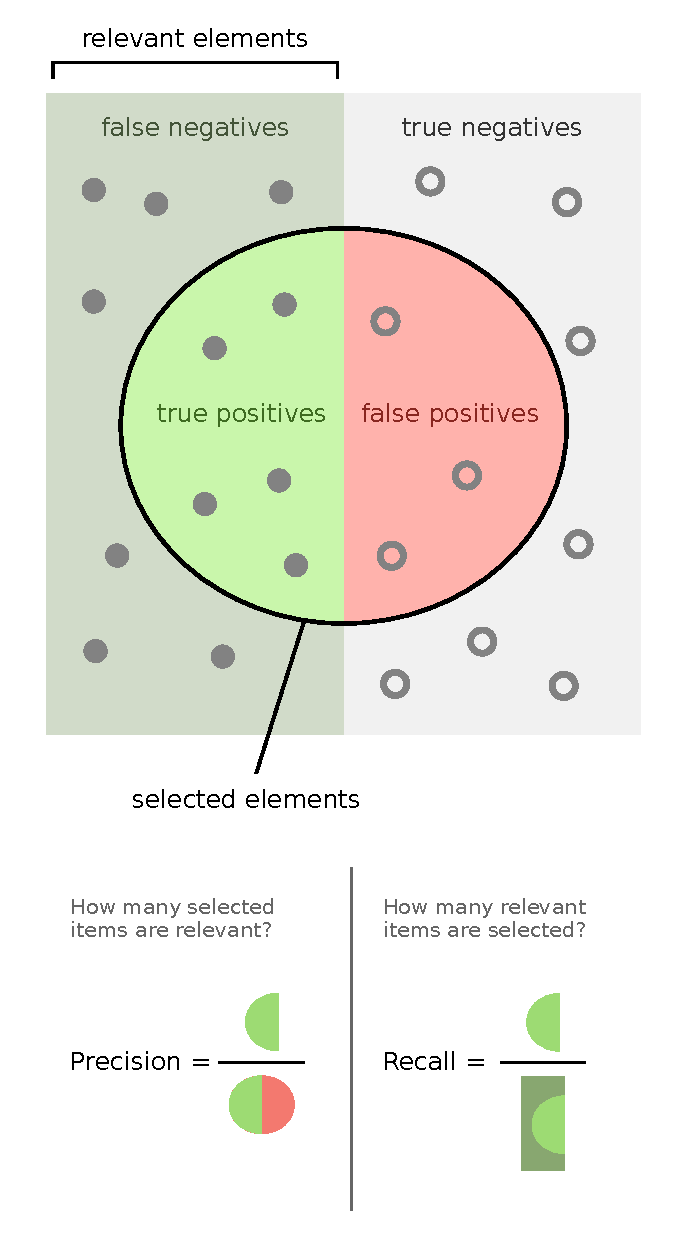
\includegraphics[height=0.5\textheight]{figures/chap-4/precision-recall.pdf}
    \caption{Visual representation of the relationship between precision and recall. Illustration originally proposed on the Wikipedia's page on Precision and Recall.}
    \label{processing:precision-recall}
\end{figure}

The F1-Score corresponds to the harmonic mean of the Precision and Recall.
\[2\cdot \frac{precision\cdot recall}{precision + recall}\]

However, NER evaluation also involves predicting the location of the entity in the sentence.
Consequently, there are many ways to obtain results partially correct.
Hence, conferences such as CoNLL defined a variant of the F1-Score better suited for this task \parencite{tjongkimsangIntroductionCoNLL2003Shared2003}.
It redefines the three previous metrics as follows:

\begin{itemize}
    \item Precision is the percentage of predicted entity name tokens that line up exactly with the tokens in the evaluation data.
          If the whole entity is not retrieved by the method, its Precision is zero.
    \item Recall the percentage of entities that appear at exactly the same location in the predictions.
    \item F1 score remains the harmonic mean of the Precision and Recall.
\end{itemize}

In the context of disaster response, \emph{Recall} is the preferred metric, as missing out reports or relevant information due to excessive filtering might be detrimental to the system.

% \subsubsection{Semi-supervision evaluation}
% Semi-supervised learning suffers from a lack of standard evaluation metrics.
% Therefore, we propose a set of metrics to evaluate that aspect.
% The core of semi-supervised learning is to leverage a small amount of labeled data among a larger volume of unlabeled ones to perform the task.
% The first metric to measure the effect of label propagation is the number of entities that have received a label through the label propagation.
% This metric allows for evaluating the "range" of the label propagation within the unlabeled dataset.
% The second metric of interest to evaluate the efficiency of the label propagation on the given problem is to measure how many entities labeled through the propagation have contributed to the final performances.
% % Propagation Efficiency = entities labeled through propagation

\subsection{Results}
% ! Évaluer avec différentes seeds.
This section presents the results of the evaluation of the method presented, using the
parameters mentioned and the datasets presented.
First, the performances of the NER are reported.
Then the performances of the semi-supervision.
Finally, the last part is dedicated to investigating the interest of dimension reduction in the setup.

The Figure~\ref{processing:fire-example} provides a visual of the result of the method, where the semantic cluster related to fire is displayed.

\begin{figure}[htb]
    \centering
    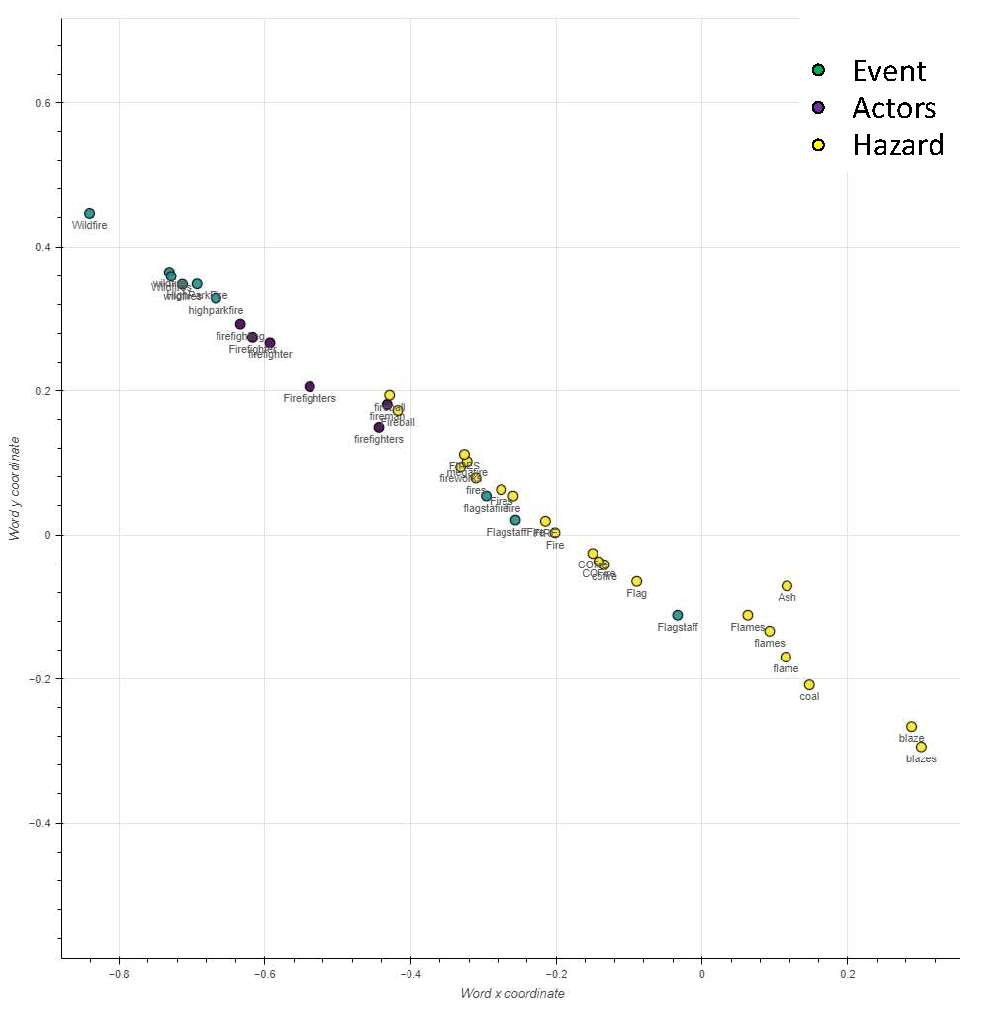
\includegraphics[width=\textwidth]{figures/chap-4/fire-example.pdf}
    \caption{2D projection of the semantic cluster related to \textit{fire} after label propagation. The projection is obtained using UMAP.}
    \label{processing:fire-example}
\end{figure}

% ? Comme l'approche s'appuei essentiellement sur des KW, elle renvoit forcément un haut recall.
% ? Ce n'est pas tellement génant dans notre cas, étant donné qu'il s'agit d'un système de support
% ? et non d'automatisation de la prise de décision.
% ? Si quelques entités sont taggés de la mauvaise manière, cela aura peu d'importance d'un
% ? point de vue de l'opérateur.

\subsubsection{NER performances}
% ! Compare with https://github.com/napsternxg/TwitterNER
The performances of our method over all types of events are reported in Table~\ref{table:overall-results}

\begin{table}[bht]
    \centering
    \caption{Results on the four types the events.}
    \begin{tabular}{rcccc}
        Category     & Precision & Recall & F1\-Score & Support \\
        \toprule
        Environment  & 0.220     & 0.652  & 0.328     & 69      \\
        Event        & 0.643     & 0.647  & 0.645     & 434     \\
        Actors       & 0.040     & 0.333  & 0.071     & 3       \\
        Hazard       & 0.263     & 0.764  & 0.391     & 89      \\
        Equipements  & 0.176     & 0.600  & 0.273     & 5       \\
                     &           &        &           &         \\
        weighted avg & 0.531     & 0.663  & 0.565     & 600     \\
        \bottomrule
    \end{tabular}
    \label{table:overall-results}
\end{table}

The performances for each type of disaster are reported as well.
The method obtains its best results on the Event class (see Table~\ref{table:earthquake-results}, Table~\ref{table:fire-results},Table~\ref{table:hurricane-results}) except for the flooding event (Table~\ref{table:flood-results}).
The method performed poorly on the flood event because the labeled terms were not matching the ones used during the event.
However, the same terms applied to the hurricane dataset provided much better performances if one compares both weighted average F1-Score.
The Environment class is partially retrieved over all datasets.
The three remaining classes — Actors, Hazard and Equipements — are harder to evaluate, as there are very little data to explore.
The only significant one is the Hazard class in the fire event, where there are 74 occurrences.
The model correctly labeled a significant part of the entities in this case.

\begin{table}[bp]
    \centering
    \caption{Result on the Earthquake event.}
    \begin{tabular}{rcccc}
        Category     & Precision & Recall & F1\-Score & Support \\
        \toprule
        Environment  & 0.132     & 0.417  & 0.200     & 12      \\
        Event        & 0.920     & 0.939  & 0.929     & 98      \\
        Actors       & 0.000     & 0.000  & 0.000     & 1       \\
        Hazard       & 0.000     & 0.000  & 0.000     & 5       \\
        Equipements  & 0.000     & 0.000  & 0.000     & 0       \\
                     &           &        &           &         \\
        weighted avg & 0.791     & 0.836  & 0.806     & 116     \\
        \bottomrule
    \end{tabular}
    \label{table:earthquake-results}
\end{table}

\begin{table}[bp]
    \centering
    \caption{Result on the Fire event.}
    \begin{tabular}{rcccc}
        Category     & Precision & Recall & F1\-Score & Support \\
        \toprule
        Environment  & 0.333     & 0.857  & 0.480     & 14      \\
        Event        & 0.651     & 0.719  & 0.683     & 57      \\
        Actors       & 0.071     & 1.000  & 0.133     & 1       \\
        Hazard       & 0.698     & 0.905  & 0.788     & 74      \\
        Equipements  & 0.000     & 0.000  & 0.000     & 0       \\
                     &           &        &           &         \\
        weighted avg & 0.640     & 0.829  & 0.713     & 146     \\
        \bottomrule
    \end{tabular}
    \label{table:fire-results}
\end{table}

\begin{table}[bp]
    \centering
    \caption{Result on the Flood event.}
    \begin{tabular}{rcccc}
        Category     & Precision & Recall & F1\-Score & Support \\
        \toprule
        Environment  & 0.183     & 0.591  & 0.280     & 22      \\
        Event        & 0.291     & 0.228  & 0.256     & 101     \\
        Actors       & 0.000     & 0.000  & 0.000     & 1       \\
        Hazard       & 0.000     & 0.000  & 0.000     & 8       \\
        Equipements  & 0.111     & 1.000  & 0.200     & 1       \\
                     &           &        &           &         \\
        weighted avg & 0.252     & 0.278  & 0.242     & 133     \\
        \bottomrule
    \end{tabular}
    \label{table:flood-results}
\end{table}

\begin{table}[bp]
    \centering
    \caption{Result on Hurricane event.}
    \begin{tabular}{rcccc}
        Category     & Precision & Recall & F1\-Score & Support \\
        \toprule
        Environment  & 0.250     & 0.714  & 0.370     & 21      \\
        Event        & 0.641     & 0.702  & 0.670     & 178     \\
        Actors       & 0.000     & 0.000  & 0.000     & 0       \\
        Hazard       & 0.015     & 0.500  & 0.029     & 2       \\
        Equipements  & 0.400     & 0.500  & 0.444     & 4       \\
                     &           &        &           &         \\
        weighted avg & 0.590     & 0.698  & 0.629     & 205     \\
        \bottomrule
    \end{tabular}
    \label{table:hurricane-results}
\end{table}

As mentioned in the definition of the metrics used, the results are only a static view of the method.
However, the method does not aim to remain static and is intended to evolve with the situational awareness of the users.
So, while these results provide valuable hints on the model's performance, it does not depict the performances of the model in suitable conditions.

% \subsubsection{Semi-supervised learning}

\subsubsection{Influence of the dimension reduction}
An additional experiment has been conducted to test the influence of the dimension reduction to evaluate how this step influences the performances.
All the parameters are kept the same, except that the dimension is never performed anywhere during training or inference.
The results are displayed Table~\ref{table:overall-results-nodim}.
The performances slightly increased, from 0.565 to 0.571 weighted average F1-score.
This version performs better on the Environment category (0.409 from 0.328 weighted average F1-score) and the Event category (0.721 from 0.645 weighted average F1-score).
Notably, there is a trade between the Precision and the Recall in this case.
For the Environment category, Precision went from 0.643 to 0.792 while Recall diminished from 0.652 to 0.275.
A similar trend is observed for the Event category, where the Precision went from 0.263 to 0.862.
However, the loss of Recall is less severe (from 0.647 to 0.620).
Maybe most importantly, this change in the model made it unable to identify Hazards (0.0 weighted average F1-score) while its counterpart was able to label some of the tokens.

\begin{table}[bht]
    \centering
    \caption{Results of our method \textbf{without dimension reduction} over the four types the events.}
    \begin{tabular}{rcccc}
        Category     & Precision & Recall & F1\-Score & Support \\
        \toprule
        Environment  & 0.792     & 0.275  & 0.409     & 69      \\
        Event        & 0.862     & 0.620  & 0.721     & 434     \\
        Actors       & 0.000     & 0.000  & 0.000     & 3       \\
        Hazard       & 0.000     & 0.000  & 0.000     & 89      \\
        Equipements  & 0.500     & 0.200  & 0.286     & 5       \\
                     &           &        &           &         \\
        weighted avg & 0.719     & 0.482  & 0.571     & 600     \\
        \bottomrule
    \end{tabular}
    \label{table:overall-results-nodim}
\end{table}

These results call for more investigations on this aspect, but it hints that different models may perform differently based on the dimensions fed to the clustering algorithm.

\section*{Conclusion}
This chapter presented a novel approach to process social media, based on machine learning, that aims to be used in disaster response situations to provide the information expected by decision-makers.
The first part discussed the context of disaster response and how it influences the processing of social media data.
In particular, it discusses the use of supervised machine learning in the context of disaster response.
This part highlighted both the advantages and disadvantages of this approach.

The second part of this chapter presents the model itself, details the functioning of its different parts and the motivation behind the choices made.
The resulting algorithm is composed of 4 steps:

\begin{enumerate}
    \item Generation of the word vectors associated with each token.
    \item Dimension reduction of the vector space obtained previously to facilitate the following clustering.
    \item Identification of semantic clusters present in the vector space using a clustering algorithm.
    \item Label propagation within the different semantic clusters.
\end{enumerate}

As of today, there is little evidence that traditional machine learning approaches are suited for such context.
Consequently, the model is designed to quickly adapt the results to fit as much as possible to the ongoing event.
In a sense, the model aims to fit the context, not the data provided initially.
The overall composition of the model is then designed with practicability in mind over raw performances.

The last section of the chapter explored the performances above.
The attempt was to explore the different aspects of the approach and quantify their impact on performances.
Improvements can be thought for several aspects of the model.
Currently, the approach is limited as it accounts for independent tokens only.
However, this issue can be solved by considering the surrounding tokens through a window sliding over the sentence.
Another aspect linked to label propagation is that semantic clusters of interest that do not contain a labeled word are currently ignored.
This aspect represents an exciting avenue for future work.
I want to emphasize that the evaluation of machine learning models, or other related systems, using the standard practices of the NLP domain, can hardly evaluate the true performances of these systems in the context of disaster response.
Evaluation on a given, the fixed dataset does not represent the unexpected and evolving nature of the problem they try to address.
\textcite{halseSimulatingRealtimeTwitter2019} proposed a tool to simulate a stream of tweets from a dataset based on message sending information.
If this tool was originally designed for training social media operators, an adapted version could be used to test machine learning algorithms dynamically.
This area remains open to contributions that will undoubtedly yield important outcomes for crisis management organizations.
Finally, the algorithm presented here has only solved a sub-part of the initial problem.
The objective of automatically retrieving information from social media cannot answer the initial challenge.
Improving disaster indeed asks for better decision-making of the different actors involved.
Similarly, improved decision-making requires better access to quality information.
However, if decision-makers informational needs might help improve the quality of the information delivered, the accessibility falls out of scope.
As described in the previous chapter, information retrieval is rarely performed by decision-makers themselves but more often by dedicated operators.
Hence the final research question: \textit{How should be organized social media processing systems in disaster management situations?}
The next chapter explores the challenges and possibilities in designing an information system for disaster response.

%%% Local Variables:
%%% mode: latex
%%% TeX-master: "../ma-these"
%%% End:
